\documentclass{article}
\usepackage[utf8]{inputenc}

\title{Introduction to High Performance Computing}
\author{Maximilian Georg Kurzawski}
\date{27.01.2023}
\usepackage{graphicx}

\usepackage{listings}
\begin{document}

\maketitle

\section{Exercise 1 - List, Tuples, array, and NumPy}

\subsection{What is the advantage of using Lists vs. Tuples}

Lists are dynamic arrays that let us modify and resize the data. 
Tuples on the other hand are static arrays whose contents are fixed and immutable. 
If you append to a list, it will allocate a new area in the memory, and move the original list there, it performs in O(1). 
You can also append to a tuple, this operation is performed as a concatenation of tuples and it performs with O(n). 
If you want to modify a tuple, you have to create a new tuple with the modified values.

\subsection{What is the advantage of using the array module vs. Python lists?}

The array module is a container that can hold a fixed number of items, and these items must all be of the same type. 
It is more efficient in terms of memory usage and performance than lists. 
The array module is more efficient because it is implemented in C, and it uses a contiguous block of memory to store the items. 
The items are stored one after the other, so the array module knows the location of each item, and it can access them directly. 
This is why the array module is more efficient than lists. 
The array module is also more efficient than lists because it can only store items of the same type. 
The array module uses the same amount of memory for each item, so it can store more items than lists, which store each item with a different amount of memory.


\subsection{What are the memory fragmentation problem and Von-Neumann bottleneck? How do they affect the performance of a code? How can we try to address it?}

The memory fragmentation problem is the problem of the memory being fragmented into small pieces, and the memory manager is not able to find a contiguous block of memory large enough to store the data. 
The Von-Neumann bottleneck is the problem of the CPU not being able to fetch the data from the memory fast enough. 
This problem is caused by the fact that the CPU and the memory are connected by a bus, and the bus has a limited bandwidth. 
This problem affects the performance of a code by causing the CPU to wait for the data to be fetched from the memory. 
We can try to address this problem by increasing the bus bandwidth, or by increasing the amount of memory. 
We can also try to decrease the amount of memory fragmentation by using a memory manager that is able to find contiguous blocks of memory, and by using a memory allocator that is able to defragment the memory.


\subsection{What is a page fault? What is the difference between a minor and a major page fault?}

A page fault is an exception that occurs when the CPU tries to access a memory page that is not in the memory.
A minor page fault occurs when the CPU tries to access a memory page that is not in the memory, but the memory manager is able to find a free page in the memory to store the data. 
In contrast the major page fault occurs when the memory manager is not able to find a free page in the memory to store the data.
When a major page fault occurs, the memory manager has to evict a page from the memory, and then it can store the data in the memory.


\subsection{What is the impact of a cache miss on the performance?}

A cache miss occurs when the CPU tries to access a memory page that is not in the cache. 
When a cache miss occurs, the CPU has to wait for the data to be fetched from the memory, or even from the disc. 
This affects the performance of the code because the CPU has to wait for the data to be fetched from the memory. 
This is why we should try to minimize the number of cache misses.


\subsection{Which HPC libraries does your NumPy installation use? Hint: you can check by writing a simple code.}
The HPC libraries that my NumPy installation uses are:

\begin{itemize}
\item openblas64__info
\item blas_ilp64_opt_info
\item openblas64__lapack_info
\item lapack_ilp64_opt_info
\end{itemize}
These were the HPC libraries that my NumPy installation uses. 
To check this, I used the following code:
\begin{lstlisting}
    import numpy as np
    print(np.show_config())
\end{lstlisting}


\section{Exercise 2 - STREAM Benchmark in Python to Measure the Memory Bandwidth}

% display all 3 pictures
\begin{figure}[h]
\centering
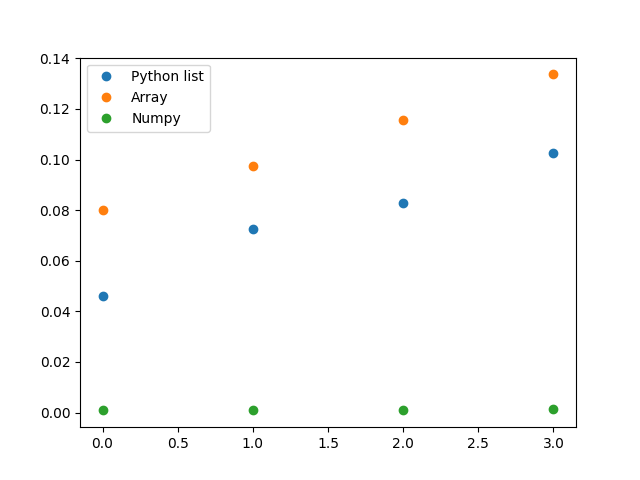
\includegraphics[width=0.5\textwidth]{1000000.png}
\caption{STREAM Benchmark Results - 1 Million}
\end{figure}

\begin{figure}[h]
\centering
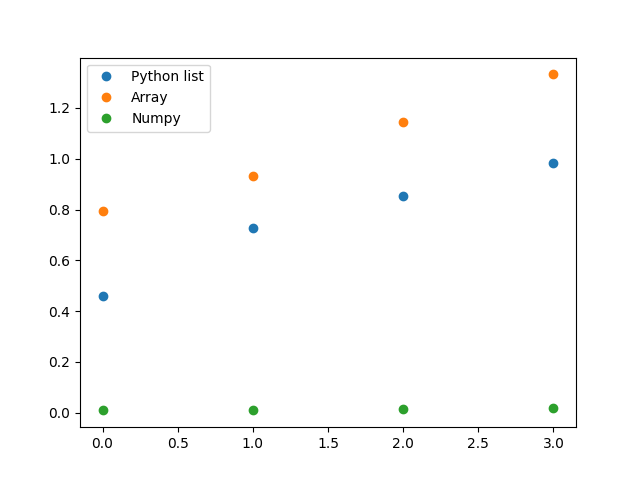
\includegraphics[width=0.5\textwidth]{10000000.png}
\caption{STREAM Benchmark Results - 10 Million}
\end{figure}

\begin{figure}[h]
\centering
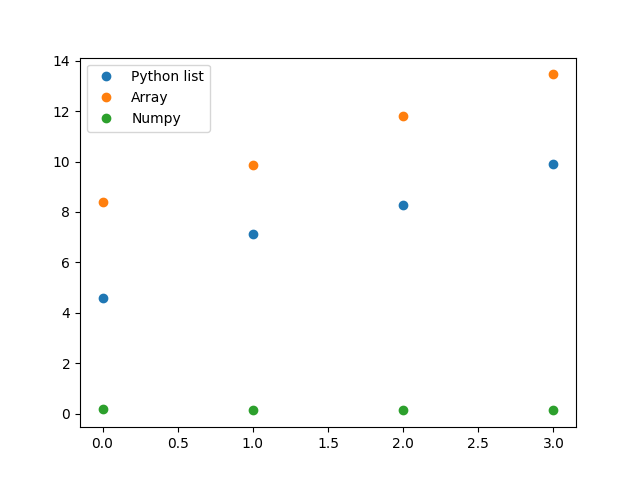
\includegraphics[width=0.5\textwidth]{100000000.png}
\caption{STREAM Benchmark Results - 100 Million}
\end{figure}

%Answer to the questions
%  How does the bandwidth vary when increasing the STREAM_ARRAY_SIZE and why?
The bandwidth varies when increasing the STREAM_ARRAY_SIZE because the bandwidth is proportional to the size of the array.
For all of the results: the bandwidth of the Python list is the lowest, the bandwidth of the Array is the second lowest, and the bandwidth of the NumPy array is the highest.

\section{Exercise 3 - PyTest with the Julia Set Code}

This is the test code for the Julia Set code:
\begin{lstlisting}
import pytest
@pytest.mark.parametrize("desired_width,max_iterations", [(1000, 300), (1000, 1000), (10000, 300), (100, 100)])
def test_julia_set(desired_width, max_iterations):
    # In order to achieve this we returned the output variable.
    import JuliaSet as js
    output = js.calc_pure_python(desired_width=1000, max_iterations=300)
    assert sum(output) == 33219980
\end{lstlisting}
As you can see for 3.2 we used the pytest.mark.parametrize decorator to test the Julia Set code with different parameters.


\section{Exercise 4 - Python DGEMM Benchmark Operation}

\subsubsection{For which kind of problems do you use the BLAS libraries?}

One uses the BLAS libraries for problems that involve matrix multiplication, and for problems that involve linear algebra.
BLAS libraries are highly tuned for performance. 
They are also easy to use.

\subsubsection{What is the difference between BLAS level-1, level-2 and level-3?}

BLAS level-1 is the simplest level of BLAS.
It is used for vector-vector operations.
BLAS level-2 is used for matrix-vector operations.
BLAS level-3 is used for matrix-matrix operations.


% dgemm double-precision dense matrix-matrix multiplication

\subsection{Measure the execution time for each approach varying the size of the matrix. Report the average and error (std. deviation or min/max or interval of confidence). Answer the question: how the computational performance varies with increasing the size of the matrices and why so?}

Here are the results for the DGEMM benchmark operation:
\begin{lstlisting}
    Average time for array size:  50
    Numpy average time:  0.019524256388346355
    List average time:  0.019973119099934895
    Array average time:  0.01978898048400879
    Numpy standard deviation:  0.0161988019210983
    List standard deviation:  0.01712826601838285
    Array standard deviation:  0.016751529326259916
    Average time for array size:  100
    Numpy average time:  0.23694856961568198
    List average time:  0.17482391993204752
    Array average time:  0.17079544067382812
    Numpy standard deviation:  0.19394822375290166
    List standard deviation:  0.13921506985460658
    Array standard deviation:  0.13796664580452822
    Average time for array size:  150
    Numpy average time:  0.5743474165598551
    List average time:  0.5775994459788004
    Array average time:  0.5648147265116373
    Numpy standard deviation:  0.47600947175501684
    List standard deviation:  0.49428629664933804
    Array standard deviation:  0.4662991817964516
    Average time for array size:  200
    Numpy average time:  1.364508867263794
    List average time:  1.4190724690755208
    Array average time:  1.3160467147827148
    Numpy standard deviation:  1.1521688895650994
    List standard deviation:  1.2162573643440988
    Array standard deviation:  1.1110624743584603
\end{lstlisting}

% how the computational performance varies with increasing the size of the matrices and why so?
The computational performance varies with increasing the size of the matrices because the computational performance is proportional to the size of the matrices.
The computational performance of the NumPy array is the highest, the computational performance of the Array is the second highest, and the computational performance of the Python list is the lowest.

% calculate Flops/s
\subsubsection{Calculate the Flops/s for each approach.}

The ammount of FLOPs can be calculated for each array size using the following formula:
\begin{equation}
    FLOPS = 2 * N^3
\end{equation}
where N is the size of the array.
This results in these FLOPS values:
\begin{itemize}
    \item array size:  50, FLOPS:  125000
    \item array size: 100, FLOPS:  2000000
    \item array size: 150, FLOPS:  3375000
    \item array size: 200, FLOPS:  6400000
\end{itemize}
To calculate the Flops/s for each approach, we can use the following formula:
\begin{equation}
    Flops/s = FLOPS / time
\end{equation}
This results in these Flops/s values:
For Approach using numpy:
\begin{itemize}
    \item array size:  50, Flops/s:  6.452213581502256e+06
    \item array size: 100, Flops/s:  8.456655341569153e+06
    \item array size: 150, Flops/s:  5.86158766211901e+06
    \item array size: 200, Flops/s:  4.700520412733408e+06
\end{itemize}
For Approach using lists:
\begin{itemize}
    \item array size:  50, Flops/s:  6.279273737621226e+06
    \item array size: 100, Flops/s:  11.460815920013299e+06
    \item array size: 150, Flops/s:  5.831359680297444e+06
    \item array size: 200, Flops/s:  4.5058934535707475e+06
\end{itemize}

For Approach using arrays:
\begin{itemize}
    \item array size:  50, Flops/s:  6.316115830078326e+06
    \item array size: 100, Flops/s:  11.703580386807087e+06
    \item array size: 150, Flops/s:  5.961116375030808e+06
    \item array size: 200, Flops/s:  4.864849510306772e+06
\end{itemize}

\subsubsection{Plot the results.}

\begin{figure}[h]
    \centering
    \includegraphics[width=0.5\textwidth]{numpy.png}
    \caption{Numpy}
    \label{fig:numpy}
\end{figure}





\section{Exercise 5 - A Python Discrete Fourier Transform}


\section{Exercise 6 - Experiment with the Python Debugger}

Advantages of using a debugger:
\begin{itemize}
    \item Debugging Code: Debuggers allow you to identify and fix bugs in your code by allowing you to step through your code and inspect the state of the program at any given point.
    \item Improving Code Understanding: Debuggers provide an interactive way to understand how your code is executing and can help you to understand how different parts of your code are interacting with each other.
    \item Time-Saving: Debuggers allow you to quickly find and fix bugs in your code, which can save you time compared to manual debugging techniques such as print statements.
    \item Debugging in Real-Time: Debuggers allow you to debug your code in real-time, giving you immediate feedback on what is happening in your code as it executes.
\end{itemize}





\end{document}
